\documentclass[tikz,border=2pt]{standalone}
\usepackage[utf8]{inputenc}
\begin{document}
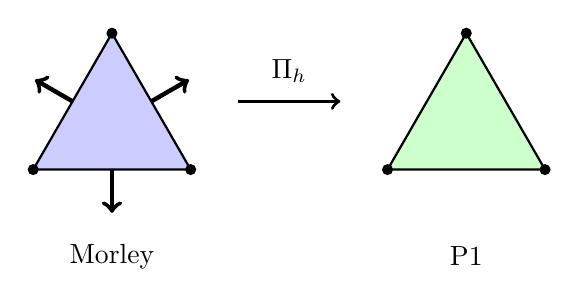
\begin{tikzpicture}

    % Morley Element - vertex values and edge normal derivatives
    \begin{scope}[shift={(0,0)}]
        \filldraw[fill=blue!20, draw=black, thick] (0,0) -- (2,0) -- (1,1.732) -- cycle;
        % Outward normal derivative averages at the edge midpoints
        \draw[->, ultra thick, black] (1,0) -- (1,-0.55);
        \draw[->, ultra thick, black] (1.5,0.866) -- (1.976,1.141);
        \draw[->, ultra thick, black] (0.5,0.866) -- (0.024,1.141);
        % Point values at the vertices
        \foreach \p in {(0,0), (2,0), (1,1.732)} \fill[black] \p circle (2pt);
        \node at (1,-1.1) {Morley};
    \end{scope}

    % Reduction operator
    \begin{scope}[shift={(0,0)}]
        \draw[->, very thick, black] (2.6,0.866) -- (3.9,0.866);
        \node at (3.25,1.25) {$\Pi_h$};
    \end{scope}

    % P1 Element - vertex values
    \begin{scope}[shift={(4.5,0)}]
        \filldraw[fill=green!20, draw=black, thick] (0,0) -- (2,0) -- (1,1.732) -- cycle;
        \foreach \p in {(0,0), (2,0), (1,1.732)} \fill[black] \p circle (2pt);
        \node at (1,-1.1) {P1};
    \end{scope}

\end{tikzpicture}
\end{document}
